This chpater demonstrates the use of machine learning in beacon tracking using 
an unmanned ground vehicle (UGV) and a WiFi-enabled microcontroller such as the 
ESP32.

\section{Assets}
\begin{enumerate}
    \item UGV chassis with DC motors
    \item ESP32 microcontroller with Type-B USB cable
    \item L293D Motor Driver IC
    \item Breadboard and Jumper Wires
    \item Android phone
    \item (Optional) USB 2.0/3.0 Hub
\end{enumerate}

\section{Procedure}
\begin{enumerate}
    \item Make the connections as per the wiring diagram in Fig. \ref{fig:beacon}.
    \item Connect the ESP32 board to your Android Phone.
    \item Generate the firmware by entering the following commands.
        \begin{lstlisting}
$ cd codes
$ pio run
        \end{lstlisting}
    \item Go to ArduinoDroid and select
        \begin{lstlisting}
Actions - Upload - Upload Precompiled
        \end{lstlisting}
    and choose the firmware file at
        \begin{lstlisting}
codes/.pio/build/firmware.hex
        \end{lstlisting}
    \item Now put the phone at a reasonable distance from the UGV with no 
    obstacles in the way and then turn on the hotspot. The UGV should travel
    towards the phone and stop near it.
\end{enumerate}

\begin{figure}[!ht]
    \centering
    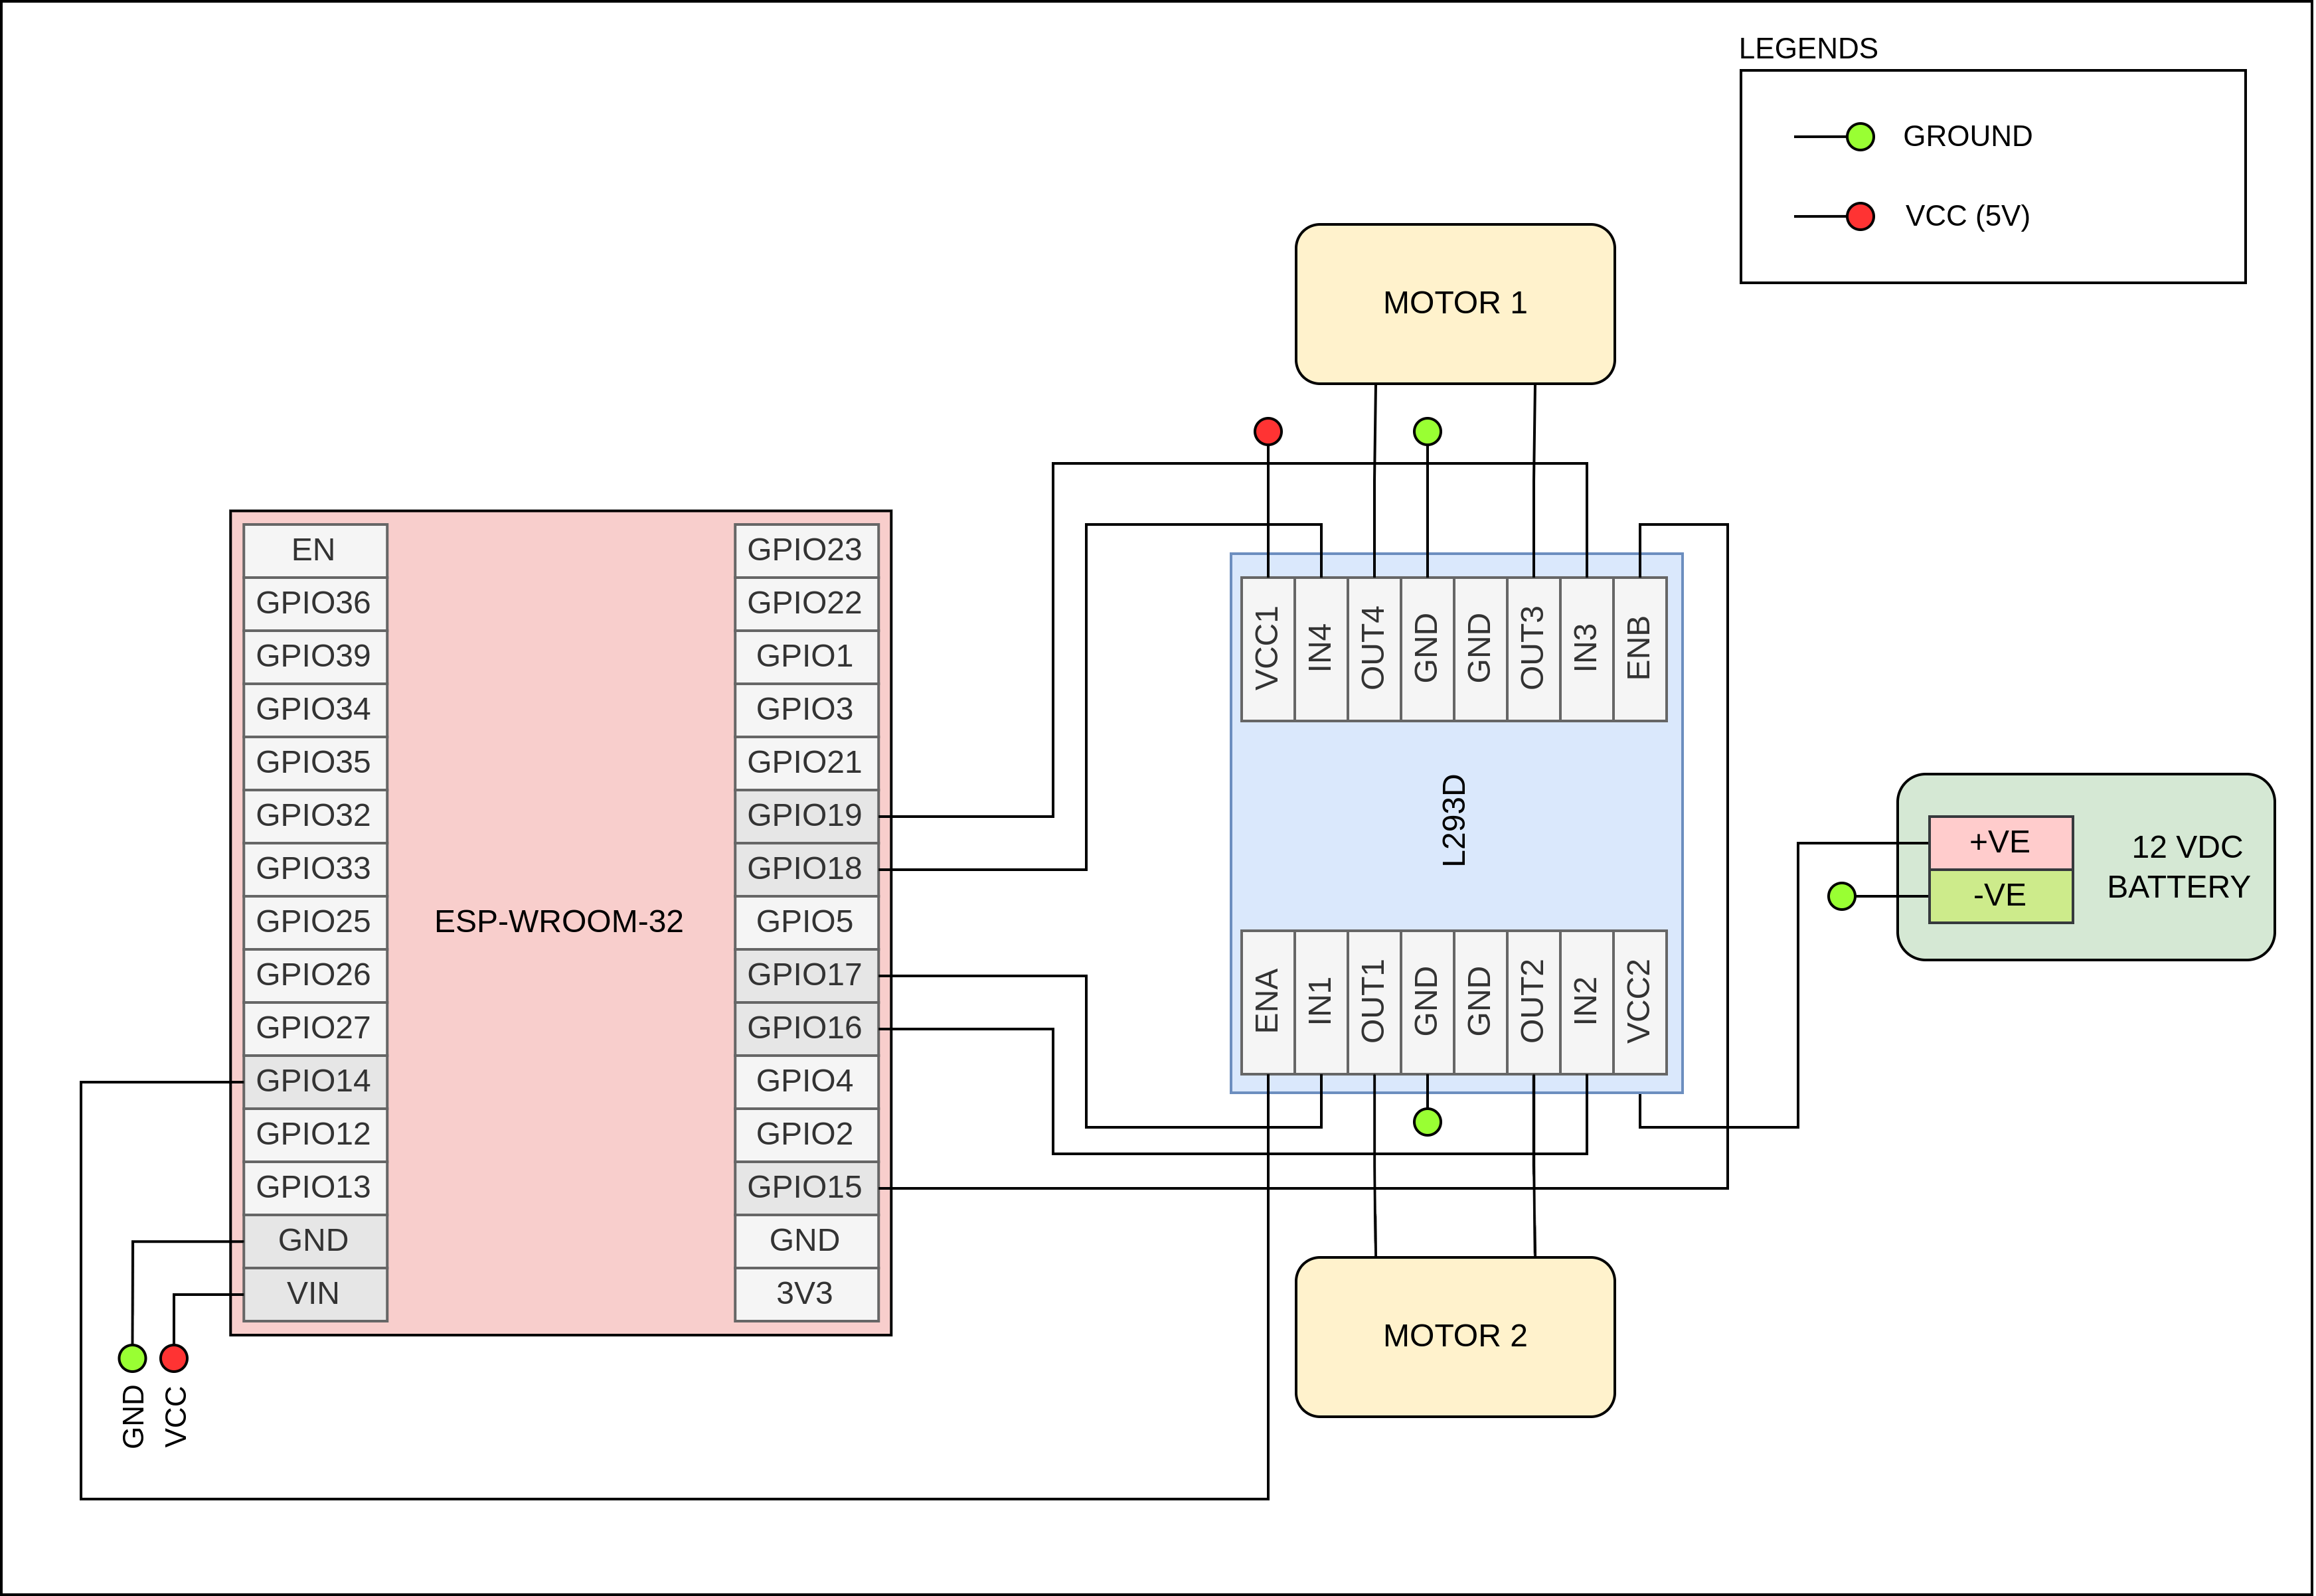
\includegraphics[width=\columnwidth]{ugv-beacon/figs/beacon.png}
    \caption{Wiring Diagram for Beacon Tracking.}
    \label{fig:beacon}
\end{figure}

\section{Working}
\subsection{Underlying Principles}
\begin{enumerate}
    \item To estimate (radial) distance to beacon, we use its signal strength.
        For WiFi, this is the \textbf{Received Signal Strength Indicator} (RSSI).
    \item The RSSI ($R$ dBm) at distance $d$ metres is given by
    \begin{align}
        R(d) = R(1) - 10\log_{10}\brak{d}
    \end{align}
    \item Clearly, $R(d)$ is a convex function. Hence, we can use gradient 
    descent.
\end{enumerate}

\subsection{Algorithm Description}
Please note that this is a generic description of the algorithm employed. Refer to
\begin{lstlisting}
ugv-beacon/codes/src/main.cpp
\end{lstlisting}
for a more verbose implementation.
\begin{enumerate}
    \item If the UGV is close enough to the beacon, \textit{terminate}.
    \item Take measurements at various points on a straight line.
    \item Based on these measurements, decide the next move of the UGV, and 
    recurse till the UGV is close enough to the beacon.
\end{enumerate}

\section{Observations}
\begin{enumerate}
    \item The UGV eventually converges close to the beacon (here, the hotspot).
    \item However, if there are a lot of nearby obstacles, the UGV may not 
    converge close to the location of the beacon. It may either get physically 
    blocked by the beacon or the signal interference may be too high.
\end{enumerate}
